\section{Understanding data geometry}
We are given a dataset $D = \{ (x_i, y_i) \quad i = 1, 2, \dots, n \}$ with $x_i$ being the flattened image and $y_i$ the label taking values in $\{ 0, 1, \dots, 9 \}$.

\begin{figure}[H]
    \centering
    % First image
    \begin{minipage}{0.14\textwidth}
        \centering
        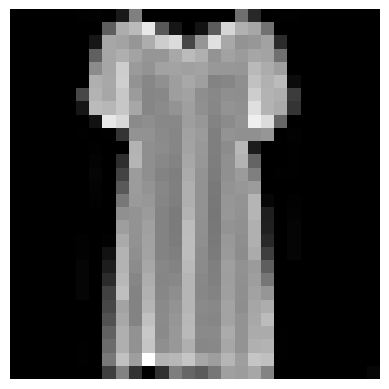
\includegraphics[width=\textwidth]{figures/dress.png}
    \end{minipage}
    % Second image
    \begin{minipage}{0.14\textwidth}
        \centering
        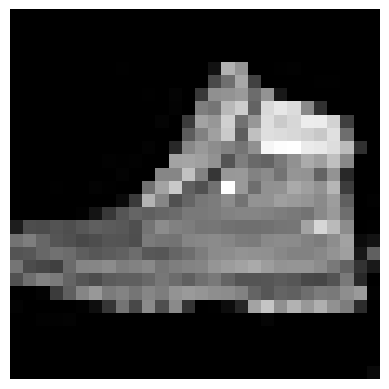
\includegraphics[width=\textwidth]{figures/shoe.png}
    \end{minipage}
    % Third image
    \begin{minipage}{0.14\textwidth}
        \centering
        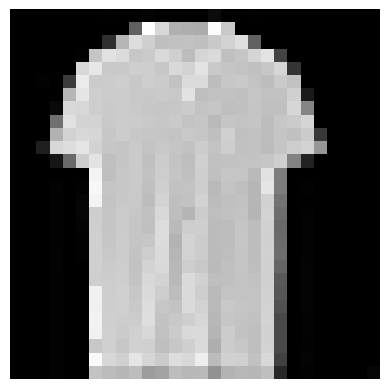
\includegraphics[width=\textwidth]{figures/tshirt.png}
    \end{minipage}
    \caption{Three samples from the dataset corresponding to the categories: dress, ankle boot and T-shirt.}
\end{figure}


\subsection{Data preparation}
Before performing PCA, it's important to center the data. In fact, it's considered best practice to not only center the data but also standardize it.
\begin{align}
    X \leftarrow \frac{X - \mu_X}{\sigma_X}
\end{align}


\subsection{Understanding PCA and KPCA}
The \textbf{Principal Component Analysis} is a linear transformation of the data that allows us to project it in a new space in which the covariance matrix is diagonal and its eigenvalues are sorted from the largest to the smallest. Selecting the first k components allows us to reduce the dimensionality of the data minimizing the information loss. \\
However, in most cases, the orignal space in which our data lies does not make it easy to disentagle it. Often, to better disentagle our data it is necessary to project it onto a bigger space, here is where \textbf{Kernel PCA} comes in. \\
The covariance matrix can be seen as a matrix of similarities in which the inner product employed is the covariance, and since we are working in a centered space, the dot product. To compute similarities in a wider space that allow us to introduce non-linearities we can use kernels.
The kernel matrix is defined as
\begin{align}
    K &= k(x_i, x_j) \quad \forall i, j
\end{align}
where $k$ is the kernel function. We then want to solve the same problem as before
\begin{align}
    K v &= \lambda v
\end{align}
where $v$ are the eigenvectors and $\lambda$ the eigenvalues. The projection is then computed as
\begin{align}
    y_k &= \sum_{k=1}^{n} \alpha_{i,k} \cdot k(\mathbf{x}_i, \mathbf{x})
\end{align}
where $\alpha_{i,k}$ are the coefficients of the $k$-th eigenvector.


\subsection{Testing multiple kernels}
Every kernel indirectly defines a Hilbert space of functions with some
properties. The tested kernels are the following:
\begin{align*}
    \mathcal{H}_{\text{gaussian}}   &= \left\{ f : \int | \hat{f}(w) |^2 e^{\frac{\sigma^2 w^2}{2}} dw < \infty \right\} \\
    \mathcal{H}_{\text{poly2}}      &= \left\{  \right\} \\
    \mathcal{H}_{\text{sigmoid}}    &= \left\{  \right\} \\
    \mathcal{H}_{\text{cs}}         &= \left\{  \right\} \\
    \mathcal{H}_{\text{laplace}}    &= \left\{ f : \int | \hat{f}(w) |^2 \frac{\gamma^2 + w^2}{\gamma} dw < \infty \right\} \\    
\end{align*}
In addition to this we enunciate the following theorem.

\begin{theorem}
Forall $i = 1, 2, \dots, M$, let $\phi_i : \mathcal{X} \rightarrow \mathcal{H}_i$ be a feature map such that 
$$
    K_i (x, y) = \langle \phi_i(x), \phi_i(y) \rangle_{\mathcal{H}_i}
$$
Then the kernel $K$ defined by
$$
    K(x, y) = \sum_{i=1}^M K_i(x, y)
$$
can be expressed as
$$
    K(x, y) = \langle \phi_S(x), \phi_S(y) \rangle_{\mathcal{H}_S}
$$
where 
$$
\phi_S : \mathcal{X} \rightarrow \mathcal{H}_S = \mathcal{H}_1 \bigoplus \mathcal{H}_2 \bigoplus \dots \bigoplus \mathcal{H}_M
$$
is the \textbf{concatenation} of the feature maps $\phi_i$:
$$
    \phi_S(x) = \left[ \begin{array}{c} \phi_1(x) \\ \phi_2(x) \\ \vdots \\ \phi_M(x) \end{array} \right]
$$
\end{theorem}

Moreover, the other following theorem allows us to understand what is
happing from a functional point of view.

\begin{theorem}
The solution $f^{\star} \in \mathcal{H}_{K_S}$ when we learn with 
$K_S = \sum_{i=1}^{M} K_i$ is equal to
$$
    f^{\star} = \sum_{i=1}^{M} f^{\star}_i
$$
where $(f^{\star}_1, f^{\star}_2, \dots, f^{\star}_M) \in \mathcal{H}_1 \times \mathcal{H}_2 \times \dots \times \mathcal{H}_M$
is the solution of
$$
    \min_{f_1, f_2, \dots, f_M} \text{R}(\sum_{i=1}^{M} f_i^n) + \lambda \sum_{i=1}^{M} || f_i ||_{\mathcal{H}_i}^2
$$
\end{theorem}
Both the theorems are taken from the slides of the course
\enquote{Machine Learning with Kernel Methods} by J. Mairal, et al.
\cite{mairal2022kernelmethods}.


In practice, this means we can define a new kernel as the sum of others
and obtain a linear separator in the space made by the concatenation of
the feature maps of the original kernels. Moreover, each kernel contribute
with its regularization term to the final solution. The sum can be generalized
to a weighted sum and in this case the regularization term is weighted as well.
We define our custom kernel as:
\begin{align*}
    K_{\text{custom}}(x, y) &= K_{\text{gaussian}}(x, y) + K_{\text{cs}}(x, y) \\
    &= e^{\gamma_1 ||x-y||^2} + \tanh( \gamma_2 \left( 1 + \frac{\langle x, y \rangle}{||x|| ||y||} \right) )
\end{align*}
where $K_{\text{cs}}$ is the kernel of the cosine similarity rescaled
in the interval $[0, 2]$ and the gamma parameters are $\gamma_1=0.5$ and
$\gamma_2=1.386$.

Notice that we are combining a kernel invariant to rigid motions with 
a kernel invariant to rotations (with respect to the origin) and scaling.
The aim is to obtain a kernel which is invariant to all these transformations.

We then compute the explained variance ratio of the kernels and we
plot it in the following figure.
\begin{figure}[H]
    \centering
    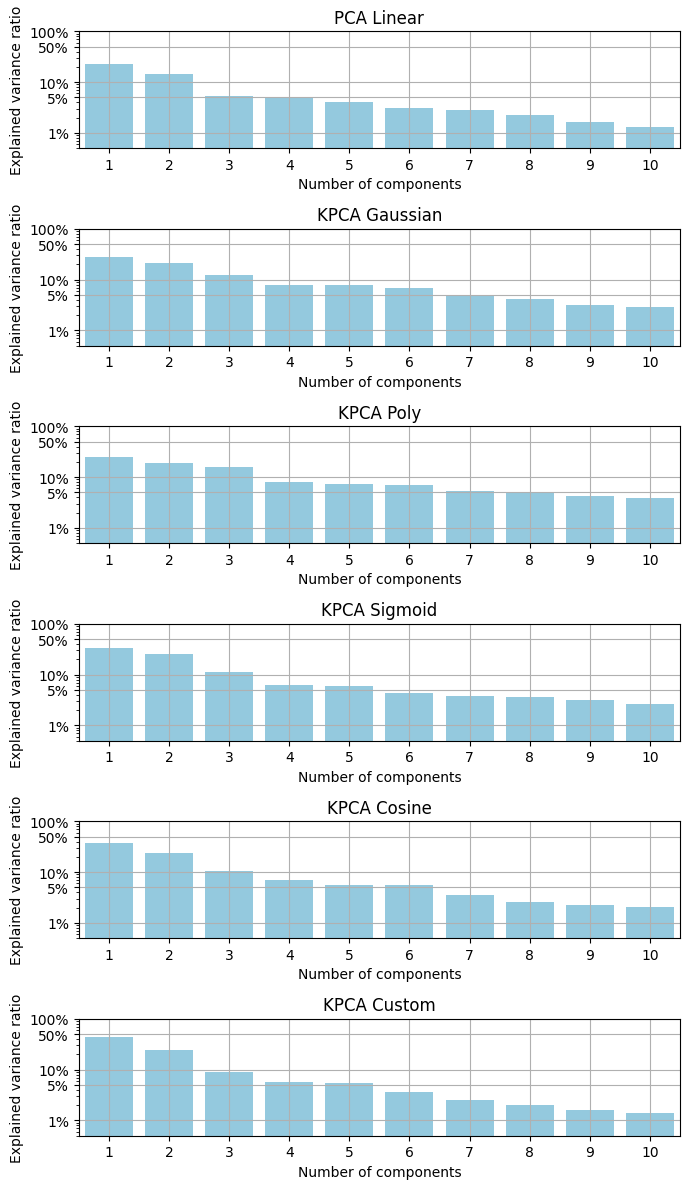
\includegraphics[width=0.4\textwidth]{figures/expvar_ratio_plot.png}
    \caption{Explained variance ratio of the kernels.}
\end{figure}

The best kernel is the one with the highest decay of the explained variance.
We proceed by computing the decay rate for each kernel as:
$$
    \text{decay}_i = \frac{\text{expvar}_{i-1} - \text{expvar}_i}{\text{expvar}_{i-1}}
$$
Then we want to compute the average decay rate of the kernels, but since we
prefer a decay rate which is higher in the first components, we weight this
average by the harmonic series.
$$
    \text{HWDR} = \frac{\sum_{i=1}^{n} \frac{1}{i} \cdot \text{decay}_i}{\sum_{i=1}^{n} \frac{1}{i}}
$$
The results are displayed in the following table.

\begin{table}[H]
    \centering
    \begin{tabular}{|c|c|}
        \hline
        Kernel      & HWDR \\
        \hline
        Linear      & 31.3 \\
        Gaussian    & 25.1 \\
        Poly2       & 20.9 \\
        Sigmoid     & 28.9 \\
        CS          & 32.8 \\
        Custom      & \textbf{38.2} \\
        \hline
    \end{tabular}
\end{table}

The custom kernel is the one with the highest HWDR, and it is the one we
will use for the rest of the analysis. We can visualize the 3D projection
of the data in the following plot.

\begin{figure}[H]
    \centering
    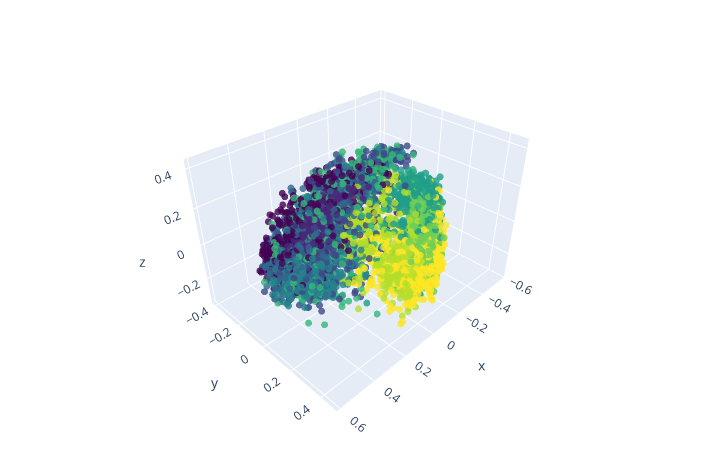
\includegraphics[
        width=0.4\textwidth,
        trim={100 10 100 90},
        clip
    ]{figures/CustomKernel3D.png}
    \caption{3D projection of the data using the custom kernel.}
\end{figure}



\section{Bridging unsupervised and supervised}

It is not always easy to retrieve labeled data, and in these cases we
can use unsupervised learning to cluster the data and then assign the
labels to the clusters.

\subsection{Clustering}
In this section we try to reconstruct the labels by solving a clustering task
and finding the best assignment of the labels to the clusters. In order
to do so we test the following clustering algorithms:
\begin{itemize}
    \item KMeans
    \item Agglomerative Clustering
    \item Gaussian Mixture Model
    \item Spectral Clustering
\end{itemize}

The choide of these algorithms is motivated by the fact that we now
a priori the number of clusters, which is the number of classes in the
dataset. We then train each algorithm on the data and compute multiple
metrics, such as the Adjusted Rand Index, the Normalized Mutual Information and
the Silhouette Score. The results are displayed in the following table.
\begin{table}[H]
    \centering
    \begin{tabular}{|c|c|c|c|}
        \hline
        Algorithm          & ARI   & NMI   & Silhouette \\
        \hline
        KMeans             & 0.342 & 0.488 & 0.228 \\
        Agglomerative      & 0.367 & 0.512 & 0.198 \\
        Gaussian Mixture   & \textbf{0.411} & \textbf{0.570} & \textbf{0.167} \\
        Spectral           & 0.379 & 0.511 & 0.213 \\
        \hline
    \end{tabular}
\end{table}

From which we can see that the Gaussian Mixture Model is the best 
performing algorithm.
To map the clusters to the labels we perform a manual inspection of the
clusters and the labels by visualizing the ten points closest to the
centroid of each cluster. We then assign the label to the cluster by
majority voting. 
Because it is not clear how to assign the couples (pullover, shirt) and (dress, coat)
we test each of the four possible assignments and we choose the one with 
the highest adjusted rand score.
In the end we obtain the following mapping:
\begin{table}[H]
    \centering
    \begin{tabular}{|c|c|}
        \hline
        Cluster & Label \\
        \hline
        0       & T-shirt/top \\
        1       & Sandal \\
        2       & Trouser \\
        3       & Pullover \\
        4       & Ankle boot \\
        5       & Bag \\
        6       & Shirt \\
        7       & Sneaker \\
        8       & Dress \\
        9       & Coat \\
        \hline
    \end{tabular}
\end{table}

\subsection{Classification}
We can now use the labels obtained from the clustering to train multiple
classifiers and compare their performance.
We consider Support Vector Machines with different kernels, a Multi Layer
Perceptron and a Convolutional Neural Network.
For both the Neural Networks a batch size of 64 was used and the training
was performed for a maximum of 150 epochs with the early stopping mechanism
of patience 10 epochs.
The optimizer is Adam with the following hyperparameters:
\begin{itemize}
    \item Learning rate: $10^{-4}$
    \item $\beta_1$: 0.9
    \item $\beta_2$: 0.999
    \item $\varepsilon$: $10^{-8}$
\end{itemize}
The \enquote{Reduce lr on plateau} learning scheduler is used with a factor
of 0.5 and a patience of 5 epochs.
The loss function is the cross entropy loss and the activation function
is always the ReLU function, except for the output layer where the softmax
function is used.

The MLP has 4 hidden layers, each with 128 neurons.

The CNN has 3 convolutional blocks composed by:
\begin{itemize}
    \item 2D Convolutional Layer with kernel size 2, stride 1 and padding 1
    \item Batch Normalization Layer
    \item Activation Layer
    \item Max Pooling Layer with kernel size 2 and stride 2
\end{itemize}
The filters are 16, 32 and 64 respectively. In the end there are 2 fully
connected layers with 64 neurons each.

The hyperparameters have been chosen manually following the guidelines
described in \textit{Deep Learning} by Goodfellow, et al. \cite{goodfellow2016deep}.



The results are displayed in the following table.
\begin{table}[H]
    \centering
    \begin{tabular}{|c|c|c|}
        \hline
        Model          & Training Accuracy & Validation Accuracy \\
        \hline
        SVM (Linear)   & 16.3 & \textbf{10.0} \\
        SVM (Poly)     & 18.8 & 7.3 \\
        SVM (Gaussian) & \textbf{20.4} & 6.5 \\
        SVM (Sigmoid)  & 10.4 & 8.6 \\
        MLP            & \textbf{20.4} & 5.9 \\
        CNN            & 16.3 & \textbf{10.0} \\
        \hline
    \end{tabular}
\end{table}
Where the training accuracy is computed on the labels obtained from the
clustering and the validation accuracy is computed on the original labels of 
the validation set.


\section{Fully Supervised Learning}

In this section we avoid learning the labels from the clustering and we
directly train the classifiers on the original labels. We test them on
both the KPCA reduced dataset and the original dataset.

\subsection{KPCA reduced dataset}
We train the same classifiers as before on the KPCA reduced dataset and
we compare the results with the ones obtained in the previous section.
The results are displayed in the following table.
\begin{table}[H]
    \centering
    \begin{tabular}{|c|c|c|}
        \hline
        Model          & Training Accuracy & Validation Accuracy \\
        \hline
        SVM (Linear)   & 78.0 & 76.4 \\
        SVM (Poly)     & 80.1 & 77.1 \\
        SVM (Gaussian) & 83.6 & 81.1 \\
        SVM (Sigmoid)  & 65.2 & 64.5 \\
        MLP            & \textbf{87.1} & \textbf{82.5} \\
        CNN            & 85.4 & 79.1 \\
        \hline
    \end{tabular}
\end{table}

As we can see, the performance of the classifiers definitely improved
when trained on the original labels.

\subsection{Original dataset}
We repeat the same experiment on the original dataset and obtain the
following results.
\begin{table}[H]
    \centering
    \begin{tabular}{|c|c|c|}
        \hline
        Model          & Training Accuracy & Validation Accuracy \\
        \hline
        SVM (Linear)   & \textbf{100.0} & 80.4 \\
        SVM (Poly)     & 89.6 & 83.2 \\
        SVM (Gaussian) & 90.8 & 84.6 \\
        SVM (Sigmoid)  & 79.0 & 77.3 \\
        MLP            & 93.9 & 85.0 \\
        CNN            & 96.9 & \textbf{86.4} \\
        \hline
    \end{tabular}
\end{table}
We can see that the performance of the classifiers improves even more
when trained on the original dataset. We should also note that no 
tuning of the hyperparameters was performed in this section and we 
just used the same hyperparameters as in the previous section.
By tuning them for this dataset we could obtain even better results.


\section{Conclusions}
In this report we have seen how Kernel PCA can be used to reduce the
dimensionality of the data and how it can outperform PCA when the data
lies in a non-linear manifold.
We have also seen how unsupervised learning can be used to retrieve
labels from the data and how these labels can be used to train classifiers.
Finally, we have seen how the performance of the classifiers can improve
when trained on the original labels.